\documentclass[12pt]{report}
\usepackage[T1]{fontenc}
\usepackage[utf8]{inputenc}
\usepackage{amsmath,amssymb,amsfonts} % Required for some math elements, equation environment and inline $ (math) $
\usepackage{makeidx}
\usepackage{graphicx} % Required for the inclusion of images
\usepackage{txfonts}
%\usepackage{times} % Uncomment to use the chosen font 
\usepackage[skip=5pt,font={small,it},labelfont=bf]{caption}
\usepackage{subcaption}
\usepackage{siunitx} % Provides the \SI{}{} and \si{} command for typesetting SI units 
\usepackage{color}
\usepackage[english]{babel} %%% SPRAWDZANIE PISOWNI EN
%\usepackage[polish]{babel} %%% SPRAWDZANIE PISOWNI PL

%%% PAGE HEADERS COMMANDS %%%
\usepackage{fancyhdr} % Page Headers and Footers
\pagestyle{fancy} %page style with FancyHDR package
\fancyhf{} % clear the header/footer style
\lhead{\leftmark} % hdr left - standard marking (chapter names)
\rhead{\thepage} % hdr right - page numbering
%\setlength{\textwidth}{14cm}
\setlength{\textheight}{20cm} 

% BIB REF COMMANDS
\usepackage[nottoc,notlot,notlof]{tocbibind}
\usepackage[backend=bibtex,style=numeric,sorting=none]{biblatex}  
\addbibresource{references.bib}

%Bibliography sorting options 
%option	description
%nty	sort by name, title, year
%nyt	sort by name, year, title
%nyvt	sort by name, year, volume, title
%anyt	sort by alphabetic label, name, year, title
%anyvt	sort by alphabetic label, name, year, volume, title
%ydtn	sort by year (descending), name, title
%none	entries are processed in citation order

% CODE LISTINGS COMMANDS
\usepackage{verbatim} % Pre-formatted text environment 
\usepackage[linesnumbered,ruled,vlined]{algorithm2e} % Algorithms with ctan algorithm2e 
\usepackage{listings}
\definecolor{mygray}{rgb}{0.4,0.4,0.4}
\definecolor{mygreen}{rgb}{0,0.6,0.4}
\definecolor{myorange}{rgb}{0.8,0.2,0}
\lstset{ 
	basicstyle=\footnotesize\sffamily\color{black},
	keywordstyle=\color{mygreen},
	commentstyle=\color{mygray},
	identifierstyle=\color{blue},
	stringstyle=\color{myorange},
	numbers=left,
	numbersep=5pt,
	numberstyle=\tiny\color{mygray},
	frame=tbTB,
	breakatwhitespace=false,         
	breaklines=true,                 
	captionpos=t,                    
	keepspaces=true, 
	columns=fullflexible,
	showstringspaces=false,
	float=t,
	tabsize=2,
	title=\lstname,
	caption=\lstname,
	language=C++
} 


%\newtheorem{definition}{Definicja} % przykład nowego środowiska 
%\newtheorem{example}{Przykład}[chapter] % przykład nowego środowiska 
%\newtheorem{corollary}{Wniosek}[chapter] % przykład nowego środowiska 

%%% TO DO notes
\usepackage[textsize=footnotesize]{todonotes}
% \usepackage[disable]{todonotes}
\newcommand{\td}[1]{\todo[inline]{TO DO: #1}}

%%% TOC HYPERLINKS %%%
\usepackage{hyperref}
% remember to use \tableofcontents after title
\hypersetup{
	colorlinks,
	citecolor=black,
	filecolor=black,
	linkcolor=black,
	urlcolor=black,
	pdftitle={Generating two-dimensional game maps with use of cellular automata}
}  

\usepackage{cleveref}

%%% STRONA TYTUŁOWA - DANE
\title{Generating two-dimensional game maps with use of cellular automata}
\author{Michał Wolski}

\begin{document}

\maketitle
\renewcommand{\contentsname}{Table of contents}
\tableofcontents  

%%%%%%%%%%%%%%%%%%%%%%%%%%%%%%
\chapter{Introduction} \label{rozdzial.wstep} 
During recent years, presence of computer games in human lives has increased. The amount of time spent on playing games by the modern society has shown that games are desirable both as a means for entertainment and a medium of expression. However, as the interest in games rises \footnote{The Interactive Software Federation of Europe compiles and publishes statistics which include frequency of gaming in European countries and show that demand for games is on the rise. \url{https://www.isfe.eu/industry-facts/statistics}} and computer games become increasingly complex, the need for game content must also rise. Elements such as believable maps, textures, sound and models (among other types of content) are a necessary resource for production of games. 

Studies such as \autocite{hendrikx2013procedural} show where the evidence for insufficiency of manual content creation may be found. In the study, authors point to work of Kelly and McCabe \autocite{kelly2007citygen}, Lefebvre and Neyret \autocite{lefebvre2003pattern}, Smelik et al. \autocite{smelik2009survey} and Iosup \autocite{iosup2009poggi} as sources which reveal game content production as a time-consuming and expensive endeavour. Hence, it is logical to conclude that information contained in studies and statistics on the topic of game development suggest that most projects aimed at creating games or simulations could benefit from seeking new or more efficient automated means of content creation.

\subsubsection{Solving the inefficiency issue}
In order to provide a solution to the inefficiency of manual content production, formal methods have emerged and are commonly referred to as \textit{procedural generation techniques}, defined by the literature as processes or methods of automatic content creation, through algorithmic mechanisms \autocite{togelius2011search} \autocite{yannakakis2015experience}.

Scientific surveys such as \autocite{hendrikx2013procedural} and \autocite{smelik2009survey} show why investigating procedural generation is useful for the game industry, by providing examples of successful methods which can be used to generate content for games. Primary concerns which drive the interest in automated ways to create game content are the rising project costs and increasing development time.

In order to reduce the cost of game development, allow for greater replay value or provide a feeling of vastness to the game worlds that designers aim to create, procedural content generation techniques can provide an attractive solution to the problem of content creation. Surveys such as \autocite{hendrikx2013procedural}, \autocite{togelius2011search} and \autocite{de2011survey} show what types of game content can be generated and are a good starting point for seeking methods of procedural generation.
 
%%%%%%%%%%%%%%%
\section{Objectives}

This thesis focuses on automated creation of 2-dimensional game maps using a cellular automata approach to generate small map tiles and merge them into a bigger map. Such approach allows for a degree of control to the map designer -- who may want to decide which tiles will be merged and at which locations in the map they will be present. Integrating manual editing or parametrization of desired results with procedural generation techniques has been proposed before in the works concerning procedural generation techniques \autocite{bidarra2010integrating}, \autocite{smelik2010integrating}, \autocite{smelik2011declarative}. 

Beginning experimentation with flat maps on 2-dimensional plane avoids the complexity that may arise when dealing with higher dimensions, hence the main aim is to develop a solution to the problem of automating planar map creation for games. 

Specifically, maps created by the generator should be planar and their layout must have characteristics of shapes that can be helpful in design of believable environments. These characteristics may include irregularity, asymmetry and imbalance. The goal is to create structures that are interesting because of their unpredictability, somewhat resembling the look of results produced by natural processes like erosion, dissolution, deformation, tectonic fragmentation or weathering.
 
%%%%%%%%%%%%%%%
\section{Thesis scope}

The research carried out to support this thesis was focused on discovery of generative techniques presented in current literature describing methods of content generation for games. 

Work on preparing the solution has been divided into the following parts, described in the remainder of this thesis:

\begin{itemize}
	\item research on procedural generation of planar maps and method selection
	\item design of a map generator program and its implementation in C++
	\item experiments to find a set of rules that generate satisfying maps
	\item extending the feature set of the generator
\end{itemize}

\td{review scope after thesis body is done >> scope well defined? scope matches content?3}

%%%%%%%%%%%%%%%
\section{Thesis structure}
This thesis includes introduction followed by three chapters. \cref{rozdzial.teoria} serves as a study on possible mechanisms that could be used for procedural generation and specifically, for creation of 2D maps for games. \cref{rozdzial.praktyka} describes design and implementation of a solution to the problem along with performed experiments. Chapter \cref{rozdzial.podsumowanie} summarizes the findings and concludes the thesis.

%%%%%%%%%%%%%%%
\section{Experimental setup}

The solution that allowed to carry out experiments in this thesis was implemented using the C++ programming language and compiled with MSVC++ 14.0 compiler, natively included in the Visual Studio 2015 Community Edition IDE. Other tools and libraries used in the project:

\begin{itemize}
	\item Dear ImGui, by Omar Cornut - to easily build an Immediate Mode user interface. Project homepage:  \url{https://github.com/ocornut/imgui}
	\item GLFW 3.2.1 library - to create an OpenGL context and have direct access to texture functions. Project homepage: \url{http://www.glfw.org/} 
	\item \td{SFML not used}
\end{itemize}  

In order to satisfy requirements for using OpenGL API function calls, it is recommended to use a dedicated graphics processing unit and install updated drivers. For the purposes of development and experiments \textit{nVidia GeForce GTX 560M } was used and drivers were updated to latest available versions.
 
This thesis has been prepared with \LaTeX\space system for document typesetting, included diagrams were drawn with \textit{UMLet} - an open source modelling program.
 

%%%%%%%%%%%%%%%
\section{Abbreviations and acronyms} 

The following terms, abbreviations and acronyms have been used in the thesis.

\begin{description} 
	\item[CA] Cellular Automaton (or Automata). A simulation consisting of cell objects.
	\item[PCG] Procedural Content Generation. An automated process of creation.   
	\item[GUI] Graphical User Interface
	\item[ASCII] American Standard Code for Information Interchange - a character encoding standard, used to represent characters in computers and information systems
	\item[RPG] Role-Playing Game
	\item[] \td{ review thesis, find unexplained acronyms }  
\end{description}

%%%%%%%%%%%%%%%%%%%%%%%%%%%%%%
\chapter{Research on 2D map generation methods} \label{rozdzial.teoria}

%%%%%%%%%%%%%%%
\section{Maps and cartography} 

Historically, maps have been used by the human race since ancient times. The need for navigation in the world has been a driving force behind the evolution of maps. Starting with cave paintings and representations of stars on the sky, our kind had the need for capturing an abstract model of a territory, terrain shape, location of useful resources or some other aspect of surrounding environment in a useful way.

Making a model of the physical (or fictional) world with maps requires choice of the data types describing locations represented on the map. List of data types visualized with maps has been growing with the evolution of cartography and whenever new technologies have been introduced to the map making crafts. Some examples of data possible to represent on maps are:
 
\begin{itemize}
	\item physical maps - terrain shape, elevation, forests, bodies of water, etc.
	\item political maps - borders around a territory, districts, states
	\item climate and weather maps - temperature, humidity, precipitation, wind currents
	\item geologic maps - terrain features, location of precious resources underground
	\item star maps - views of the distant cosmic objects measured by solid angles from a fixed point
	\item route maps - transport links, connections joining points on the modelled territory
\end{itemize}

Although early maps had the form of drawings or etchings on surface of solid materials, now there are other possibilities of representing the abstract model which a map aims to represent. The rise of digital maps and geographic information systems has opened new possibilities - maps have become dynamic entities, stored digitally, easily updated with new data and not limited to the boundaries of physical model. With digital maps, it is possible to show more than one layer of data, as chosen by the user, whereas physical maps are limited to the data and view scale chosen initially at the time when map was crafted. Despite the limitations, they still can serve well as a medium for storage of geographic information, requiring simpler processes during archival and conservation efforts \autocite{bagrow2017history}.

\begin{figure}[h!]
	\centering
	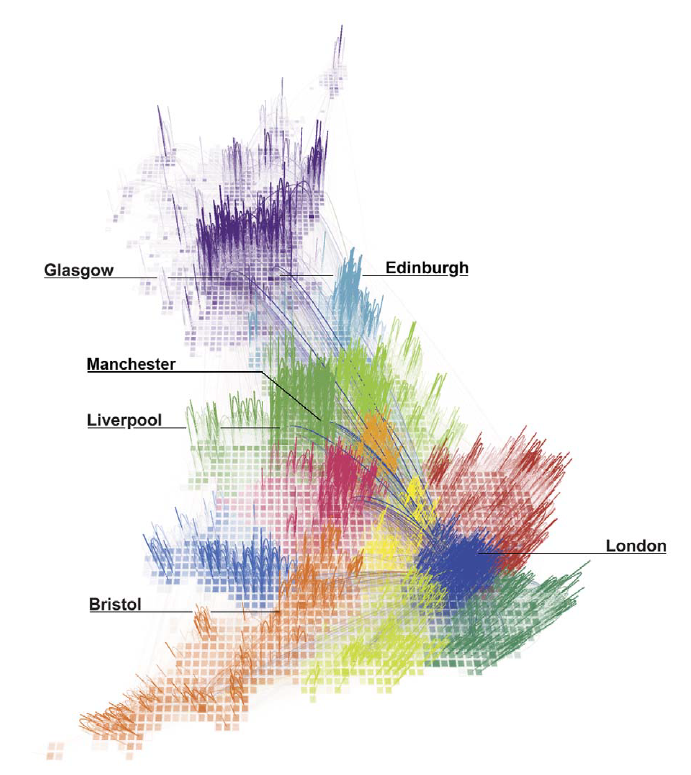
\includegraphics[width=0.6\linewidth]{images/journal_netw_talk_map}
	\caption{Pure data map showing the geography of talk in Great Britain. Authors measured the total talk time via communication networks between areas in Britain and used the data to produce the visualzation. Source article: \autocite{10.1371/journal.pone.0014248}}
	\label{fig:journalnetwtalkmap}
\end{figure}


Digital technology has also brought interesting methods to the art of crafting maps, allowing for new types of maps to be crafted, which brought previously undiscovered insights into the nature of represented territories. For example, with data maps such as the one described by article \autocite{10.1371/journal.pone.0014248} it is possible to draw more useful borders around regions, fitting actual human interaction groups as opposed to those defined by past governments, as shown in figure \cref{fig:journalnetwtalkmap}. Maps like these are generated from vast data sets, collected and stored in databases - an approach that would not be possible without use of digital technology. Since maps can emerge out of pure data, the same approach can be used to create fictional maps, out of generated data.

The possibility of visualizing map layers which could not have been created and shown without digital data processing techniques and ease of experimentation with the information and algorithms used to create modern digital maps have also made it apparent that the source data for the layer itself do not necessarily have to measure some aspect of reality, but can be generated using mathematical methods. Such approach effectively allows for creation of fictional maps, representing imaginary territories. Moving on, the next section presents examples of fictional maps and their use in games, physical and digital alike. 


%%%%%%%%%%%%%%%
\section{Maps in games} 

It is not clear what kind of game was the first one in history to use a map to represent the game world, however two notable examples may easily come into mind: Chess and Go, which are both widely known around the world. 

Chess, a board tactical war-game developed before 6th century AD, uses black-white board as the map of its world. Although the environment represented by a chess board is very simple, it has some important features and rules. The map is composed of square cells, which are arranged on 8 by 8 grid, effectively creating a rigid boundary around the game world, which according to game rules - cannot be crossed. Each cell has 8 neighbours and can be occupied by only one game piece.

Another game, originating from ancient China, defines a similar, grid-based game world, effectively making a map of a uniform planar territory. Go is played on 19 by 19 board, however smaller board sizes are used as well. In Go, the goal is to capture more territory than the opponent, which is done by placing game pieces on line intersections, one piece per turn.


\begin{figure}[h]
	\centering
	\begin{subfigure}[b]{0.4\linewidth}
		\centering
		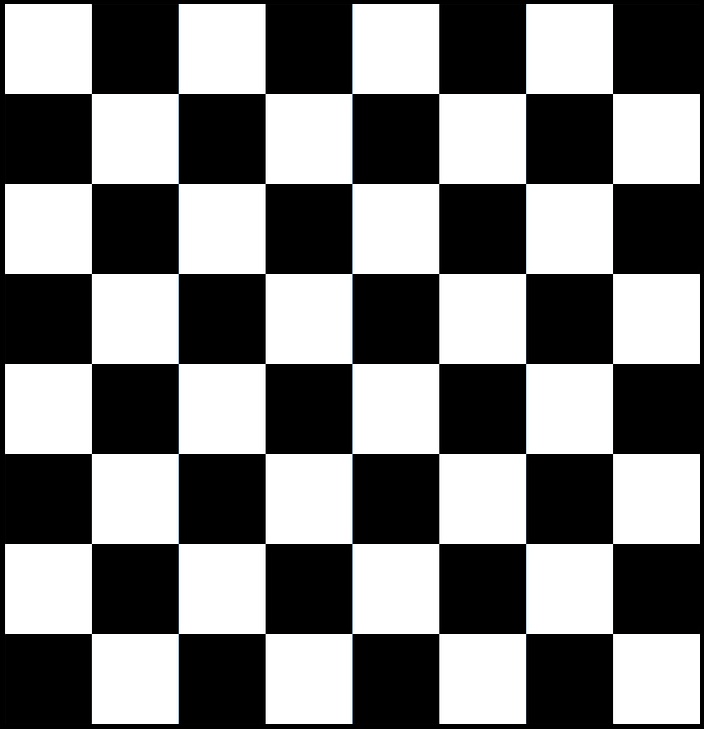
\includegraphics[width=\textwidth]{images/chessboard}
		\caption{Empty chess board} 
	\end{subfigure}
	\hfill
	\begin{subfigure}[b]{0.4\linewidth}
		\centering
		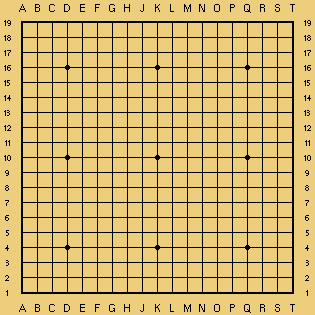
\includegraphics[width=\textwidth]{images/goboard}
		\caption{Go board during gameplay} 
	\end{subfigure} 
	\caption{Chess and Go both use planar boards divided into tiles by a square grid - simple maps to represent the environment in which game is played. Sources: Chessboard image - own work; Go board image - \url{https://senseis.xmp.net/?LargeBoards}, distributed under the terms of the Open Content License }
	\label{fig:neighborhood_types}
\end{figure}
 
Another interesting example of a game world map is the multi-player strategy board game Risk, invented in 1957 by Albert Lamorisse, where the map represents a territory divided into regions, which must be captured by players in order to win. Risk game shows how a political world map with imagined region borders can be creatively used in a game, as a resource for the players to fight over. The game of Risk has been since published in many variations. Most of them share the same gameplay goal: to capture more territory than the opponents do, which is an example of how a game might use environments represented by maps as a limited resource for players to acquire.
 
\begin{figure}[h]
	\centering
	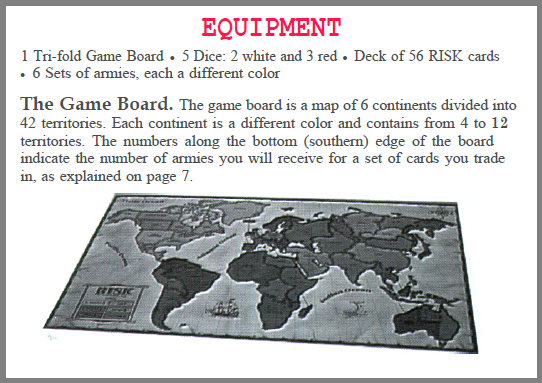
\includegraphics[width=0.5\linewidth]{images/risk-rulebook} 
	\caption{Risk rule book fragment, containing a photo of the game board. The board shows a world map with fictional political borders, dividing the map into regions, which serve as a resource for players to capture. Image source: photo taken from original Risk rule book, copyright Hasbro 1993}
	\label{fig:acrord32risk1}
\end{figure}

Modern board games have introduced many new ideas to the design of game boards. One example of such ideas is bringing modularity into the board design, composing pieces of the board similarly to how a jigsaw puzzle is composed of singular pieces. Such arrangement allows for greater value in replaying the game, since the game world can be different at each time the game is played. 

An example of such game is Carcassonne, published in 2000, designed by Klaus-Jürgen Wrede in Germany. The game of Carcassonne involves an interesting mechanism: rather than having a fixed game board, cards with tiles are used to construct the board during gameplay. The game rules around tile placement can be thought of as an algorithm of procedural generation: only one tile can be placed during each game turn, adjacent to other tiles, forming a connection with features that tiles represent - roads must connect to roads, fields to other fields, and cities to cities. The rules ensure that the players will develop the game board as the game progresses, which leads to an interesting observation: each turn, the players are presented with new territory to consider in their decisions - and since the game requires players to deploy their resources onto the constructed game map in order to accumulate score and eventually win, these decisions may often become quite challenging with increasing complexity of the board layout. There is a web version of Carcassonne available at \url{https://concarneau.herokuapp.com/game}.

\begin{figure}[h]
	\centering
	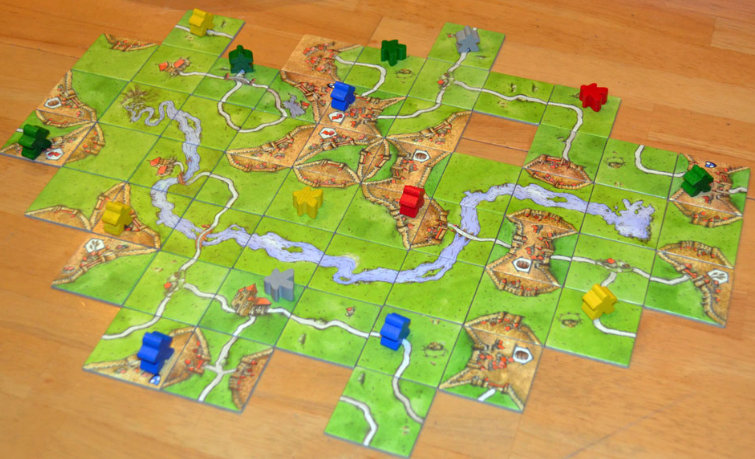
\includegraphics[width=0.7\linewidth]{images/carcassonne}
	\caption{Carcassonne game board during gameplay. Players place tiles on gameplay surface once per turn, making sure that each new tile is compatible to surrounding tiles. Image source: \url{https://deerfieldlibrary.org/2016/01/carcassonne-a-modern-board-game-for-adults-teens/}}
	\label{fig:carcassonne}
\end{figure}

There are other board games which make use of generative mechanics to create or alter the board layout, before or during gameplay. Some of them rely on randomness, while others introduce rules by which the game world may be altered. An example of such rules is presented by Labirynth, a board game designed by Max Kobbert and first released by Ravensburger company in 1986. The game board in Labirynth represents a dungeon composed of tiles representing path elements: corners, straight paths, crossings. Each turn, the game board is altered by shifting an entire row or column of movable tiles in a direction chosen by player, in effect changing the board layout.  

 \begin{figure}[h]
 	\centering
 	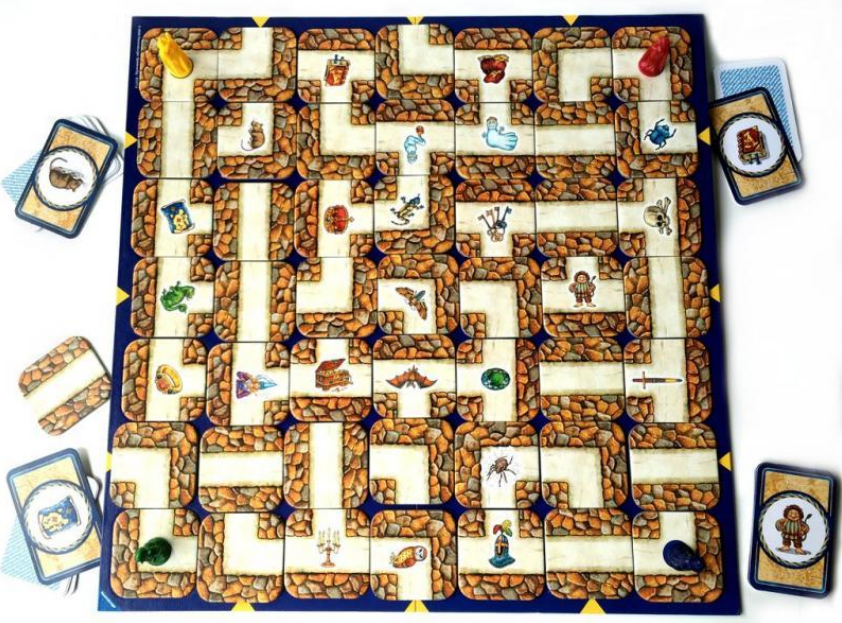
\includegraphics[width=0.7\linewidth]{images/labirynth}
 	\caption{Labirynth game board. Even rows and columns are movable (marked with a yellow triangle on board edges). Image source: \url{https://rulesofplay.co.uk/products/labyrinth} }
 	\label{fig:carcassonne}
 \end{figure}


While it is possible to find or develop interesting mechanics for board games, some more complex game rules and ideas are better implemented using computer simulation, where most of the mundane tasks which do not contribute to gameplay can be automated. Random number generation, board preparation and arrangement, checking player moves against game rules - all those activities are good candidates for automation. The other reason to simulate games may be to develop artificial intelligence algorithms which can simulate player behaviour at a chosen level of competitive play, effectively providing a way for beginners who want to learn the game they are interested in or for veterans who want to develop their skills further, as has been done for chess and other classic board games. 

Among modern board games, there are many more examples which involve interesting mechanics, but their description lies beyond the scope of this thesis project. Next section investigates a few examples of computer games and simulations, where maps are used to construct some aspects of gameplay.

%%%%%%%%%%%%%%%
\section{Interactivity and automation }

The evolution of personal computers has allowed players to enjoy a new form of entertainment - video and computer games. Possibility of performing real-time simulations on computers and development of computer graphics rendering techniques have created a new medium of expression in the form of computer software. At the time when early forms of interactive simulations were created, first computer games were also developed. 

In the past decades, when the earliest computer games have been created, an industry focused on the craft of game development has emerged. The efforts of game designers and developers have lead to creation of multiple game genres and have driven the evolution of mechanics and challenges that modern games can now offer to players.

As stated in \cref{rozdzial.wstep}, the context of this thesis does not deal with projections of 3D objects onto a plane, like the fields of geography and cartography do, as shown by works similar to \autocite{snyder1993flattening}. The goal is to generate planar maps, which makes games that include them of particular interest for finding examples of working solutions to the problem. 

Early examples involving procedurally created maps are Rogue and Nethack, dungeon crawling games developed in 1980s. Both examples generate a set of rooms with randomized dimensions, which are then connected to each other by a system of corridors, as shown in \cref{fig:nethack}.
 

\begin{figure}[h]
	\centering
	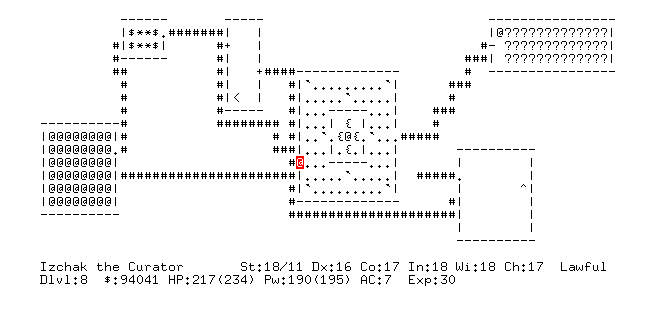
\includegraphics[width=0.7\linewidth]{images/nethack}
	\caption{An exemplary level, generated by Nethack game rules. Image source: Nethack project webpage, \url{https://nethack.org/common/index.html}}
	\label{fig:nethack}
\end{figure}

Dungeon layouts generated by Rogue or Nethack could be described as suitable for representing indoor spaces, maps produced by connecting rooms are typically do not contain irregular shapes like landmass forms found in depictions of natural terrain. It is however, possible to use such mechanisms anyway. Generated levels found in Diablo series, Torchlight, Path of Exile and a few other similar action-RPG titles suggest that careful design of map components (textures, tiles, rooms) processed later by a generation mechanism can produce believable environments, regardless of what shapes are shown by a map of their layout. 
	

%%%%%%%%%%%%%%%
\section{Existing solutions for generating planar maps}

There have been scientific surveys conducted on PCG (Procedural Content Generation) methods, which describe approaches to map generation employed in the past by successful game development projects. Contents of three such surveys are summarized in the following paragraphs.

Authors of the most general survey on PCG techniques \autocite{hendrikx2013procedural} point to other works for deeper exploration into methods involving generative grammars, genetic algorithms and hybrid approaches for generating indoor spaces. For synthesizing outdoor maps, survey lists usage of image filtering, tiling, layering, fractals, Voronoi diagrams and cellular automata. In both cases, pseudo-random number generation and hybrid approaches are listed as tools which can be helpful in finding a promising solution. 

Another general survey on PCG methods suitable for games \autocite{de2011survey} explores the subject of environmental content, listing and describing methods for generation of landscapes, continents, cityscapes, road networks and rivers. Terrain generated with methods presented in the survey has properties of naturally occurring land features with surface roughness resembling real environments. Authors list the usage of noise algorithms, L-systems, fractals and combinations of these methods along with modifications based on natural process simulations (e.g. erosion) to generate believable terrains. Described methods are categorized into \textit{assisted} and \textit{non-assisted} techniques, the former of which can be controlled by parametrization of inputs to achieve the desired outcomes and often require human support. Methods listed for generation of roads, rivers and cities involve more advanced and complicated techniques, such as the work of \textit{Chen et al.} \autocite{Chen:2008:IPS:1360612.1360702} on guiding the generation of road graphs with tensor fields, cited by the survey. Most of these methods are not suitable for this thesis project due to their complexity or are specifically designed for 3D environments.

Survey \autocite{van2014procedural} focuses specifically on generation of dungeon levels, listing and describing how cellular automata, generative grammars, genetic algorithms and constraint-based methods are used to create maps containing features of indoor spaces.

The following sections shortly discuss the possibility of applying approaches found in described surveys to generation of planar maps with irregular shapes. Since the goal of this thesis is to build a generator which performs that process, it may be worth noting the characteristics of each method described in the following sections.

\subsection{Cellular automata}
A cellular automaton (CA) is a simulation in which every object in a mathematically defined space is being updated at every step of a simulation. Historically, cellular automata and their properties have been studied since the time of first computers \autocite{Sarkar:2000:BHC:349194.349202}. One of the most complete sources on cellular automata is a book summarizing research carried out by Stephen Wolfram since 1980s \autocite{wolfram2002new}, where a classification is shown along with examples for each kind of CA. 

Specifically, 2-dimensional automata operate on a grid of cells with arbitrary discrete dimensions. Each cell in the grid has neighbours, which may be relevant to the simulation rules. Depending on the type of rules which are used by a particular CA, a different type of cell neighbourhood may be used. To present this concept concisely, a short list of definitions follows.

\begin{description}
	\item[Cell] Cells are units of state in CA simulation. Depending on CA type, they can be represented by simple values - a binary digit (0 or 1), an integer, a real or complex number with constraints, or other, more complicated value.  
	\item[Cell neighborhood] In a context of a 2D square grid of cells, neighbourhood is a collection of cells directly adjacent to the selected one.
	\item[Von Neumann neighbourhood] Includes the cell and its immediate neighbours - one to the north, south, east and west of the cell, as shown in  \cref{fig:neighborhood_types}.
	\item[Moore's neighbourhood] Includes 8 closest neighbours of the cell - immediate and diagonal, as shown in  \cref{fig:neighborhood_types}.
\end{description}
 
\begin{figure}[h]
	\centering
	\begin{subfigure}[b]{0.4\textwidth}
		\centering
		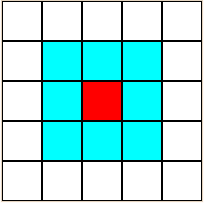
\includegraphics[width=0.5\textwidth]{images/neighborsmoore}
		\caption{Moore neighborhood} 
	\end{subfigure}
	\hfill
	\begin{subfigure}[b]{0.4\textwidth}
		\centering
		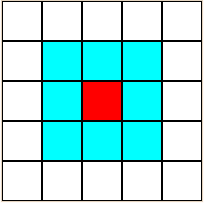
\includegraphics[width=0.5\textwidth]{images/neighborsvonneumann}
		\caption{Von Neumann neighborhood} 
	\end{subfigure} 
	\caption{Two basic types of cell neighborhood. Source: own work}
	\label{fig:neighborhood_types}
\end{figure}


Every CA simulation uses rules which drive the process of cell evolution to its next stage. Typically, such rules define how board elements must be changed once a specific cell arrangement is recognized. The set of rules must cover all possible neighbourhood patterns of a cell so that the value of each cell in a future step is unambiguous. Exemplary rules for a 2D cellular automaton are presented in  \cref{fig:examplecarules}, where included images do not cover all possible cases.


\begin{figure}[h]
	\centering
	\begin{subfigure}[b]{0.4\textwidth}
		\centering
		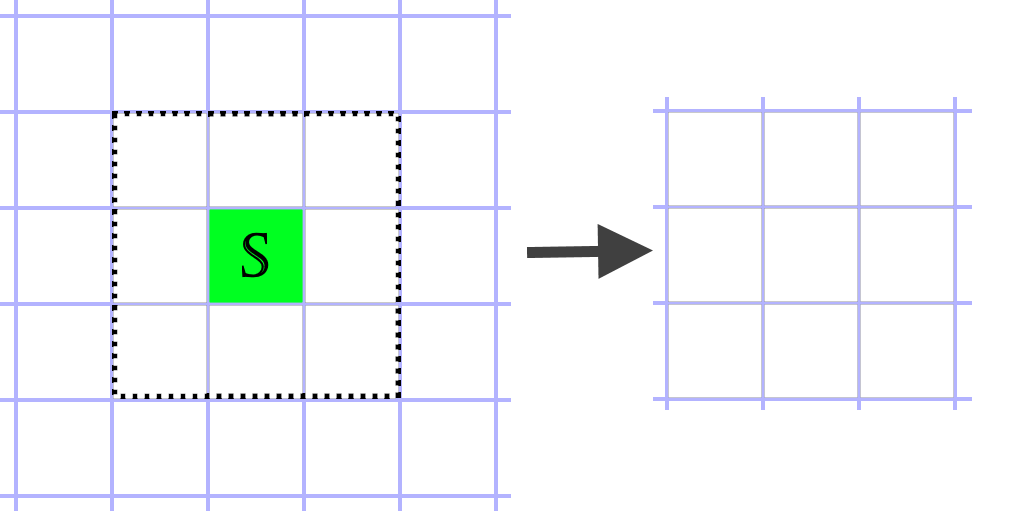
\includegraphics[width=0.5\textwidth]{images/rule0dead}
		\caption{Rule 0 - cell is set to empty when no neighbours are present} 
	\end{subfigure}
	\hfill
	\begin{subfigure}[b]{0.4\textwidth}
		\centering
		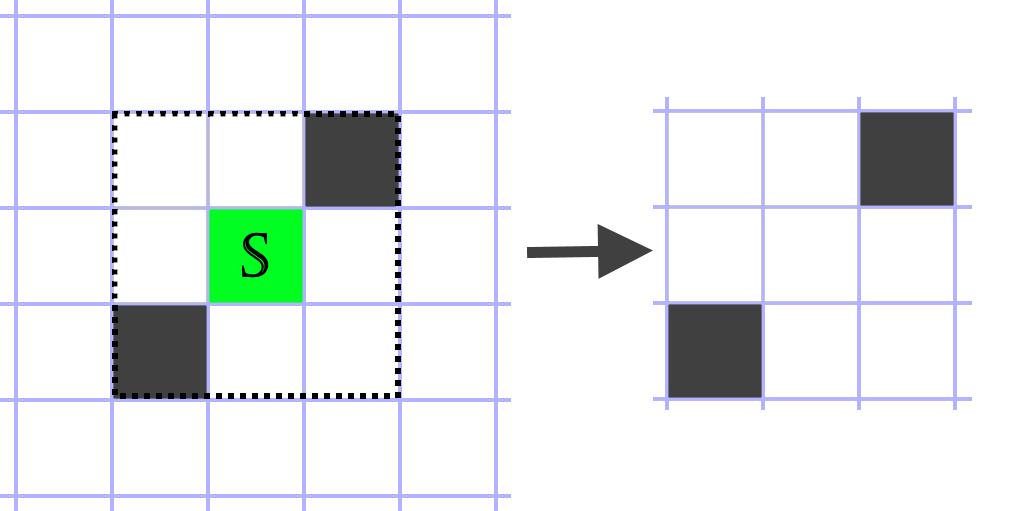
\includegraphics[width=0.5\textwidth]{images/rule2dead}
		\caption{Rule 2 - cell is set to empty if there are less than three neighbours} 
	\end{subfigure} 
	\hfill
	\begin{subfigure}[b]{0.4\textwidth}
		\centering
		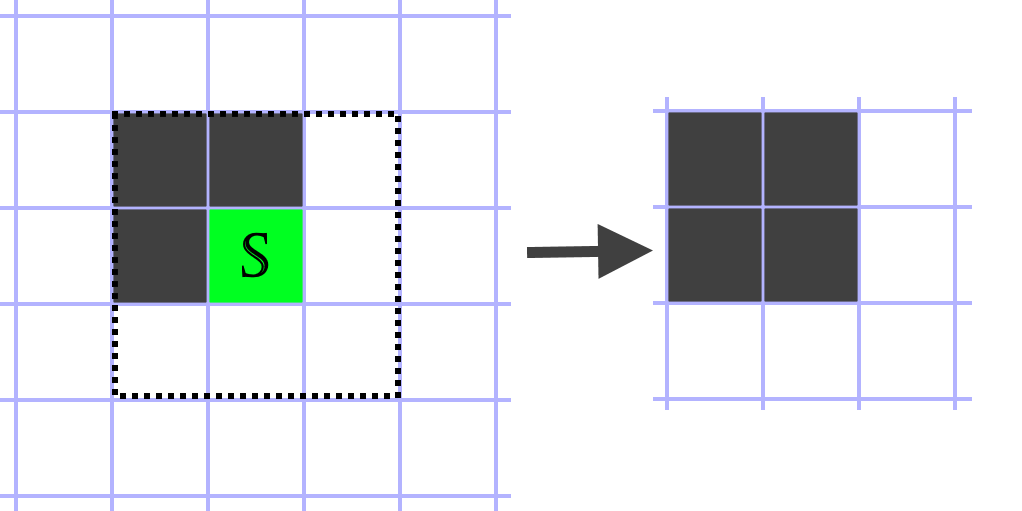
\includegraphics[width=0.5\textwidth]{images/rule3alive}
		\caption{Rule 3 - cell is set to filled if it has three neighbours} 
	\end{subfigure} 
	\hfill
	\begin{subfigure}[b]{0.4\textwidth}
		\centering
		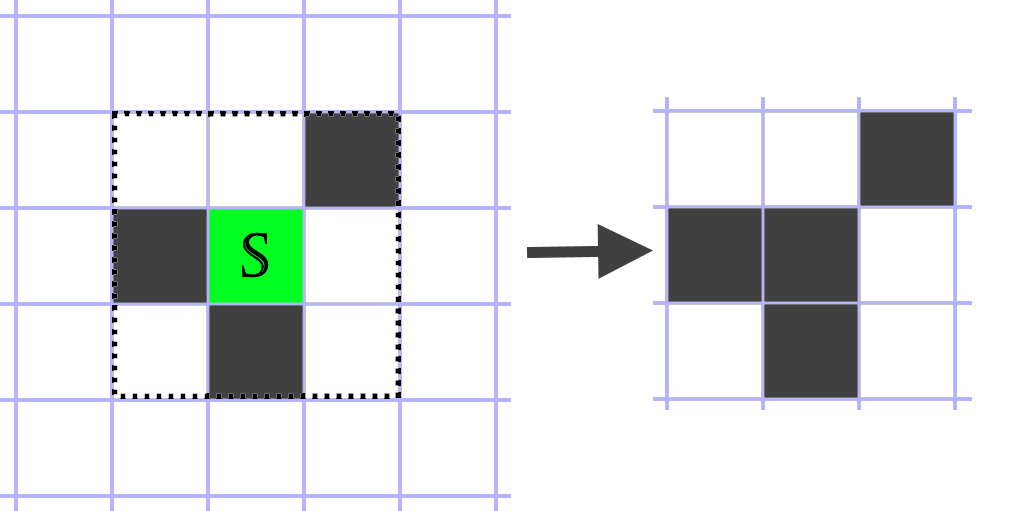
\includegraphics[width=0.5\textwidth]{images/rule3alive2}
		\caption{Rule 3a - same rule, behavior independent of neighbour positioning} 
	\end{subfigure} 
	\hfill
	\begin{subfigure}[b]{0.4\textwidth}
		\centering
		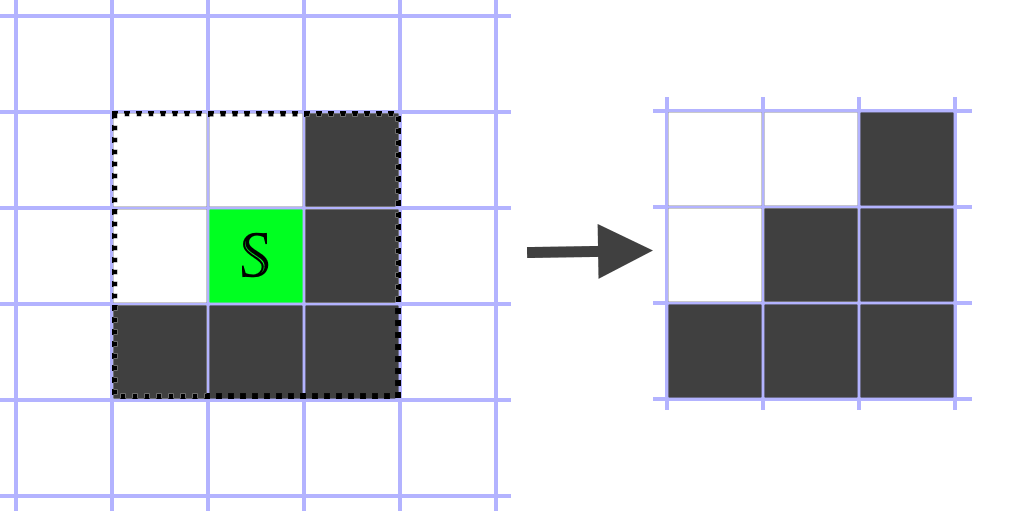
\includegraphics[width=0.5\textwidth]{images/rule5alive}
		\caption{Rule 5 - cell is set to filled if more than 3 neighbours} 
	\end{subfigure} 
	\hfill
	\begin{subfigure}[b]{0.4\textwidth}
		\centering
		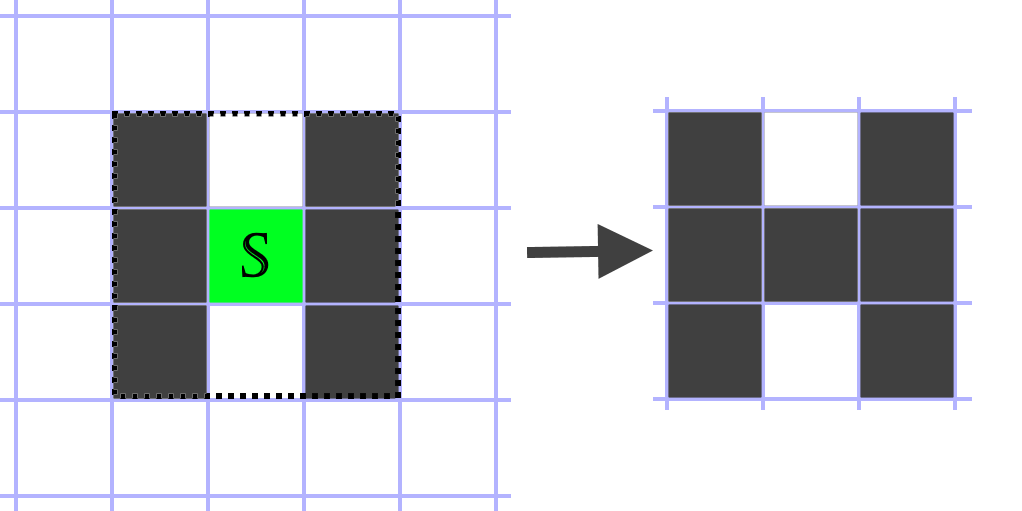
\includegraphics[width=0.5\textwidth]{images/rule6alive}
		\caption{Rule 6 - cell is set to filled if more than 3 neighbours} 
	\end{subfigure} 
	\hfill
	\caption{A subset of rules for an unknown cellular automaton which uses Moore neighbourhood. Source: own work}
	\label{fig:examplecarules}
\end{figure}

Observing the presented subset, it may be intuitive to see rules 3, 5 and 6 as alternate versions of the same rule that sets the cell state according to a simple test: 
\begin{itemize}
	\item if selected cell has less than 3 neighbours, it remains empty
	\item otherwise, it becomes filled
\end{itemize} 
However, not knowing the full set of rules for this particular automaton, it cannot be concluded if those rules can be reduced in such way. For example, there might be rules for arrangements with 4, 7 or 8 neighbours which fill the cell instead of emptying it or rules that behave differently depending on neighbour positions. Without information about the rule set, one cannot prove which properties of the cell neighbourhood are measured during simulation, nor predict the results of automaton evolution. These properties may include the following:

\begin{itemize}
	\item count of cells with state $s$ in neighbourhood,
	\item state of selected cell,
	\item state of adjacent cells (values associated with each cell),
	\item positions of neighbours with state $s$ 
\end{itemize}

An example demonstrating such difficulty in reasoning about CA rules and their consequences is one of the classic cellular automata simulations, the Game of Life\footnote{Some Game of Life simulation examples: one at MIT website \url{http://web.mit.edu/jb16/www/6170/gameoflife/gol.html} and another at \url{https://copy.sh/life/}}, invented by an American mathematician John Conway \autocite{conway1970game}. The simulation uses a square grid board, where cells can have one of two possible states: alive or dead. The rule set for Game of Life contains only three rules, based on counting alive neighbours of each cell: 

\begin{itemize}
	\item Alive cells with less than 2 alive neighbours become dead.
	\item Alive cells with 4 or more alive neighbours become dead.
	\item Dead cells with exactly 3 alive neighbours become alive.
\end{itemize}

\Cref{fig:applygol} shows an example of how these rules affect cells in a $5x5$ board during one simulation step. Cells outside the grid edges are assumed dead. 

\begin{figure}[h]
	\centering
	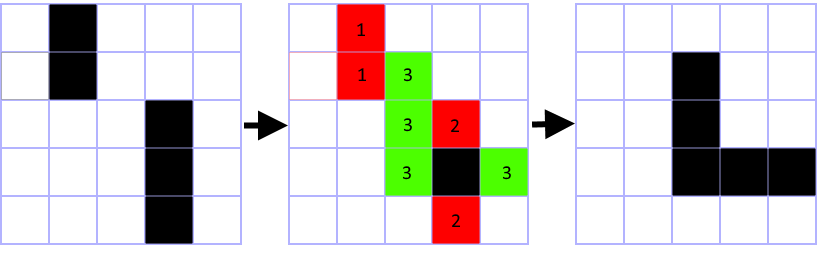
\includegraphics[width=0.7\linewidth]{images/applygol} 
	\caption{Illustration of step transition in Game of Life. Alive cells which become dead in next turn are marked red, dead cells that become alive are marked green. Coloured cells were assigned a number equal to the count of their alive neighbours. Source: own work}
	\label{fig:applygol}
\end{figure}

Despite being based on simple rules, Game of Life is able to generate complex visual patterns, such as those shown in \cref{fig:p3oscillators}. While many of such cell arrangements have been found accidentally, there are organized efforts focused on finding and cataloguing them, such as the Life Wiki at \url{http://www.conwaylife.com/wiki/}. 

\begin{figure}[h]
	\centering
	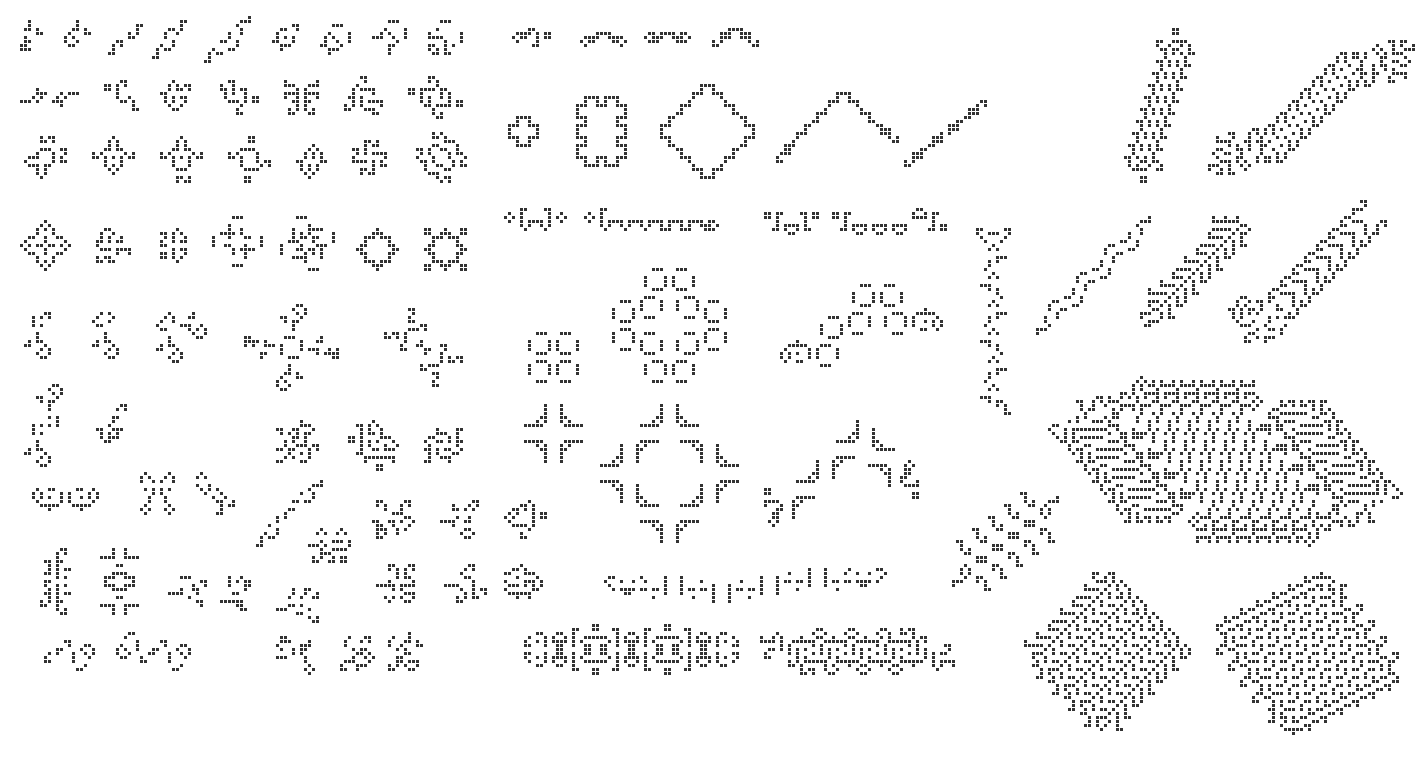
\includegraphics[width=0.9\linewidth]{images/p3oscillators}
	\caption{A collection of patterns found in Game of Life, which oscillate with period of 3 simulation steps. Image source: adapted from \url{http://copy.sh/life/?pattern=period3oscillators}}
	\label{fig:p3oscillators}
\end{figure}

Cellular automata have been used in map generation mechanisms for games, some of notable examples are Dwarf Fortress (2006),  Minecraft (Mojang, 2011) and Ultima Ratio Regum (2011). Each of these games use CA-based algorithms to generate map layers, regional structures or other types of data used to describe the game world. Examples of maps found in Dwarf Fortress and Ultima Ratio Regum show that CA-based approach to map generation can indeed yield sufficient results. Dwarf Fortress starts the generative process with randomized fractals \autocite{adams2015simulation} to define various aspects of the data layers from which the final map is built, but also uses a 3D cellular automaton to simulate behaviour of fluids (water, lava). Minecraft uses fractal noise algorithms to generate an open world map along with other methods to determine the structure of terrain layers. Also, cellular automata are utilized to simulate fluid flow and possibly to propagate updates among certain world elements (blocks with state, simulated circuits).

However, in order to develop a map generator using CA, a rule set which achieves stable board states is needed. Game of Life simulations show quick, but impermanent changes in local areas of the board, while allowing for creation of occasional stable structures. They are however somewhat rare, as \ref{fig:applygol} shows, and may be easily broken by future simulation steps, which makes them insufficient to easily compose larger structures with randomized processes.

\begin{figure}[h]
	\centering
	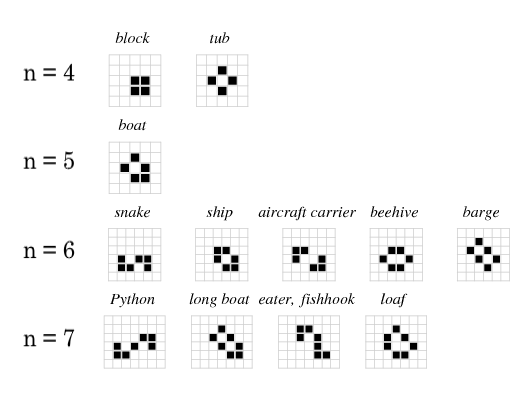
\includegraphics[width=0.6\linewidth]{images/stilllife}
	\caption{A collection of small ($n<8$, $n$ - number of cells in a pattern) still life patterns from Game of Life. Image source: adapted from \url{http://mathworld.wolfram.com/GameofLife.html}}
	\label{fig:stilllife}
\end{figure}


One of possible approaches to map generation which can create irregular shapes is the article written by L. Johnson, G. Yannakakis and J. Togelius from IT University of Copenhagen \autocite{johnson2010cellular}. Authors describe rules of a cellular automaton which is able to transform a tile filled initially with random distribution of cells into a map tile with desired properties which can later be merged with other tiles into the game map. Authors define types of cells to indicate which areas of the map are accessible (floor cells) and which are not (rock and wall cells). To achieve better control over the generation process, the following parameters can be altered: 

\begin{itemize}
	\item $r$ - percentage of floor cells in initial state,
	\item $n$ - count of CA generations (steps) to perform,
	\item $T$ - neighbourhood threshold value which defines inaccessible cells, 
	\item $M$ - Moore neighbourhood size
\end{itemize}

\td{expand on JYT10}

\subsection{Generative grammars}

Generative grammars are systems of rules that can be used to synthesize constructs of symbols, according to a given set of rules. Generative grammars have been developed in the field of linguistic theory where Noam Chomsky laid the foundations for formal grammars in the 1950s, which have been later adapted by computer science (syntax analysis algorithms, compilers, debuggers, pre-processors, post-processors, etc.).

\td{Sportelli, Francesco \& Toto, Giuseppe \& Vessio, Gennaro. (2014). A Probabilistic Grammar for Procedural Content Generation. 10.13140/2.1.3820.4163. } 

\td{Shape grammars}


\subsection{Other methods}

\td{Genetic algorithms, constraint-based, Perlin noise, others mentioned in surveys}

%%%%%%%%%%%%%%%
\section{Chosen method: cellular automata}
 
Since this thesis is focused on creation of maps through procedural processes, it is worth noting why cellular automata have been chosen as the method to develop a solution. The following arguments show why CA might be a useful approach:

\begin{itemize}
	\item as shown by \autocite{johnson2010cellular}, CA are sufficient for map generation
	\item 2-dimensional CA can be implemented in a similar way to some image processing algorithms (e.g. erosion, dilation)
	\item CA are able to model evolution of dynamical systems (e.g. fluids), which may be useful to create maps of terrain similar to natural landmass forms 
	\item amount of repetition in shapes produced by grammars depends on how complex the set of transformations is \autocite{CHOMSKY1959137}, while CA can generate surprising, chaotic results with simple rules \autocite{wolfram1984cellular}
\end{itemize}

Although grammars are favourable for clarity of transformation rules they bring to the process of map generation, CA can be a viable alternative, providing irregularity and surprise to possible results - which is why they have been chosen for experimentation in this thesis.

%%%%%%%%%%%%%%%%%%%%%%%%%%%%%%%%%%%%%%%%%%%%%%%%%%%%%%%%%%%%%%%%%%%%%%%%%%%%%%% 
\chapter{Generating and visualizing maps - proposed solution} \label{rozdzial.praktyka} 
%%%%%%%%%%%%%%%%%%%%%%%%%%%%%%%%%%%%%%%%%%%%%%%%%%%%%%%%%%%%%%%%%%%%%%%%%%%%%%% 

To describe the developed solution, this chapter consists of five sections: definition of required features, design of simple CA simulation and map generator models, followed by implementation in C++ and description of performed experiments. 

%%%%%%%%%%%%%%%
\section{Analysis of requirements for a map generator}

The approach chosen in \cref{rozdzial.teoria} can be imagined as a process that consists of several steps. Starting with generation of a board with random cell states, which after several transformations performed by CA rules becomes structured with irregular, island-like features. The resulting board is then used as one of tiles to be merged into the larger map. Each of these steps must be automated while allowing the designer a degree of control over the generation process. Transformations of the board should be applied according to parameters set by the designer, which must be constrained to ranges that do not allow creation of obviously unusable results (e.g. board filled with cells of identical state). Usable ranges of parameters can be determined with experimentation.

To formalize what map generator must do, required features and behaviours can be now extracted from the paragraph above, as follows:
 
\subsubsection{Functional requirements}

The map generator program shall perform the following functions:
\begin{itemize}
	\item prepare square tiles with random data for transformation,
	\item simulate a cellular automaton to generate irregular shapes in tiles,
	\item have a mechanism to merge tiles into a bigger map,
	\item show tile states graphically,
	\item have controls to allow tweaking CA parameters,
\end{itemize}

Optionally, the map generator program may:
\begin{itemize}
	\item have a mechanism for exporting generated maps as image files,
	\item allow manual editing of map tiles, 
\end{itemize}


\subsubsection{Operational requirements}
The map generator program shall operate with the following qualities:
\begin{itemize}
	\item real time drawing tile and map images, whenever their state changes 
	\item responsive user controls, avoid long waiting times for computation result
	\item 
	\item \td{more needed? how to extract them properly?}
\end{itemize}

%%%%%%%%%%%%%%%
\section{Design and implementation} 

In \cref{rozdzial.praktyka}, cellular automata have been chosen as a method for generating maps, so it is helpful to find resources on the topic of building cellular automata simulations. One of them is chapter 7 in Nature of Code, a book by Daniel Shiffman \autocite{shiffman2012nature}, where one can find a short tutorial on building a CA simulation. Author describes elementary concepts needed to construct a basic CA, explains how to implement a working simulation and provides helpful exercises. Another source, a book by Stephen Wolfram  \autocite{wolfram2002new} shows advanced research, exploring concepts and organizing knowledge on cellular automata.

\subsection{Basic cellular automaton}

The initial step required to implement a generator based on cellular automata is to create a framework for performing CA simulations. As stated in Nature of Code \autocite{shiffman2012nature}, a 2-dimensional CA needs the following key elements:

\begin{itemize}
	\item Cell state - every cell has a state updated on each simulation step,
	\item Grid - a space on which cells are placed,
	\item Neighbourhood - each cell needs to know the state of its neighbours to update its state.
\end{itemize}

\subsubsection{Data structures}
In order to represent state of a cell, a primitive data type is sufficient. Class model in \cref{fig:boardcell} presents an abstraction that can encapsulate a collection of cell states, along with two operations: retrieving the state of a cell in position $(x,y)$ from a grid and setting its state to a chosen value. 

\begin{figure}[h]
	\centering
	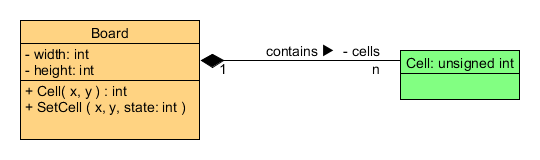
\includegraphics[width=0.8\linewidth]{diagrams/boardcell01}
	\caption{ Model of a $Board$ class, which holds cell states in its block of memory and lets its user change their states. Diagram source: own work} 
	\label{fig:boardcell}
\end{figure}

\subsubsection{Operations}
While the $Board$ class is sufficient to represent the grid of cells and their states, the concept of a neighbourhood is missing. It can be captured and represented by creating a procedure that selects a cell, and treats its neighbours as if an identifier is assigned to each of them, as shown in table \cref{tab:cellneighbors}. 

\begin{table}[h] 
	\centering 
	\begin{tabular}{| c | c | c |}\hline 
		0 & 1 & 2 \\ \hline
		7 & S & 3 \\ \hline
		6 & 5 & 4 \\ \hline
	\end{tabular} 
	\begin{tabular}{| c | c | c |}\hline 
		$(-1,-1)$ & $( 0,-1)$ & $( 1,-1)$ \\ \hline
		$(-1, 0)$ & $( 0, 0)$ & $( 1, 0)$ \\ \hline
		$(-1, 1)$ & $( 0, 1)$ & $( 1, 1)$ \\ \hline
	\end{tabular} 
	\caption{Table on left: Moore neighbourhood, with numbered cells. \textit{S} denotes cell selected as a base for further operations. Table on right: Neighbour positions, relative to selected cell $(0,0)$ Source: own work}
	\label{tab:cellneighbors}
\end{table}

In CA simulations used for map generation by \autocite{johnson2010cellular}, summing the values of cells in neighbourhood is a required operation. Hence, it is useful to include it into the $Board$ abstraction as part of its interface, which yields a class presented on \cref{fig:boardcell2} with added method for computing sum of adjacent cell values around a cell with $(x,y)$ coordinates. The $nht$ parameter can be used to control which cells are treated as neighbours.

\begin{figure}[h]
	\centering
	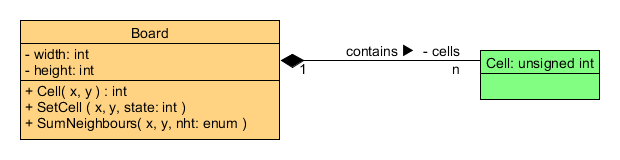
\includegraphics[width=0.8\linewidth]{diagrams/boardcell02}
	\caption{Model of a $Board$ class with a method to sum neighbour values. Diagram source: own work} 
	\label{fig:boardcell2}
\end{figure} 

\subsubsection{Implementation}
 
The model presented above is implemented by data and operations contained in the $Board$ class. It allows to simulate some basic cellular automata based on rules which require a sum of values in cells adjacent to the selected cell to decide its future state. $Board$ class methods operate as follows:

\begin{itemize}
	\item $CellAt$ can access cell at position $(x,y)$ in the grid model and return its value, as shown on \cref{lst:board-cellat},
	\item $SetCellAt$ works similarly to the previous method, accessing the cell at position $(x,y)$ and writing a new value provided by $state$ parameter, shown on \cref{lst:board-setcellat},
	\item $SumNeighbours$ computes a sum of cell values in a neighbourhood of type $nht$ at position $(x,y)$, as shown on \cref{lst:board-sumneighbourhood} 
\end{itemize}
 

\lstinputlisting[language=c, caption=Accessing cells, label={lst:board-cellat}]{listings/board-cellat.txt}
\lstinputlisting[language=c, caption=Setting cell states, label={lst:board-setcellat}]{listings/board-setcellat.txt}
\lstinputlisting[language=c, caption=Summing adjacent cell values, label={lst:board-sumneighbourhood}]{listings/board-sumneighbourhood.txt}

\subsection{Simulating CA rules} 

As described in \cref{rozdzial.teoria}, basic CA rules check the values of adjacent cells to a selected cell and determine its subsequent state. Separating the concept of a rule and its application from the cell grid structure simplifies modifying the CA rule set for further usage.

\subsubsection{Data structures}

Although applying rules to a grid of cells does not require a specialized data structure, a class to encapsulate procedures used to do so separated from $Board$ class can be useful for later development. The $Ruleset$ class presented in \cref{fig:ruleset-board} is used to produce a new board state by applying rules encoded in its internal functions, which are used by $EvolveState$ method.

\begin{figure}[h]
	\centering
	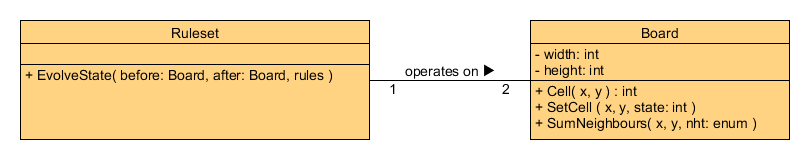
\includegraphics[width=0.9\linewidth]{diagrams/ruleset-board}
	\caption{Model of $Ruleset$ class, which is meant to use a $Board$ instance to produce a new state of the cell grid in another $Board$ instance by rewriting its cell values. Source: own work}
	\label{fig:ruleset-board}
\end{figure}

Such abstraction allows to later add an internal data structure to hold separate rules for each possible neighbourhood pattern, if needed. 

\subsubsection{Operations}

As shown in \cref{fig:ruleset-board}, the operation which handles computation of a new cell grid state is named $EvolveState()$. It does so by calling one of its internal methods chosen by $rules$ parameter. \Cref{lst:evs} shows an implemented method which calls $Board$ methods to perform the following steps:

\begin{enumerate}
	\item sum the values of cells adjacent to cell $(x,y)$,
	\item set the future $(x,y)$ cell state to 1 if the sum is less than 5,
	\item set the future $(x,y)$ cell state to 0 if the sum is more than 5.
\end{enumerate}


\lstinputlisting[language=c, caption=Applying rules to cell grid, label={lst:evs}]{listings/evolvestate.txt}

With basic CA operations organized this way, adding new rules requires implementing a new method in the $Ruleset$ class. Choosing a new set of rules is done via passing a correct parameter value to $EvolveState$ method, which can be done by binding the function call to user interface.

\subsection{Presenting the board state}

In order to visualize state of $Board$, all cell values need to be drawn as an image. To achieve this, OpenGL and ImGui libraries are used to create an environment in which it is possible to construct interface elements and render textures. 

\subsubsection{Data structures}

Before the cells can be represented as an image, their states must be converted to colour values in one of the formats interpreted by OpenGL functions. In order to do so, a class $SimpleTexture2D$ has been prepared, as shown in \cref{fig:texture}. 

\begin{figure}[h]
	\centering
	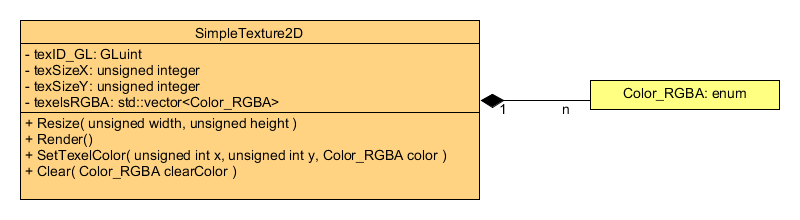
\includegraphics[width=0.9\linewidth]{diagrams/texture}
	\caption{Model of a $SimpleTexture2D$ class, which contains a collection of $Color RGBA$ elements. Source: own work}
	\label{fig:texture}
\end{figure}

Colours are represented by a 32-bit unsigned integer, with 8 bits dedicated to each colour channel (Red, Green, Blue) and additional 8 bits for the opacity (Alpha) channel, defined by type $Color RGBA$ as shown in \cref{lst:colourRGBA}. 

\lstinputlisting[language=c, caption=Definition of ColourRGBA type, label={lst:colourRGBA}]{listings/colourRGBA.txt}

\subsubsection{Operations}

Methods provided by $SimpleTexture2D$ class allow to:

\begin{itemize}
	\item set individual colour values at specified position in the $texelsRGBA$ collection, necessary for rendering the $Board$ state
	\item change the collection size, to allow support for $Board$s of different sizes,
	\item set all colour values in the collection to a specified value,
	\item request rendering of the contained data by OpenGL API.
\end{itemize}  

Such set of operations allows to achieve the goal of simple 2-dimensional image rendering, which can be used to visualize the state of all cells contained in one of the $Board$ class instances.

\subsection{Generating and merging tiles into maps}

Generating tiles for map construction is done with data and operations contained in $TileGenerator$ and $Ruleset$ classes. Internal mechanics of the $TileGenerator$ class allow it to initialize cells in the first generation to randomly selected states and then to use $Ruleset$ class to generate future states of the board. $Ruleset$ provides a set of rules which describe the possible transformations of a cell depending on the state of its neighbourhood, as described in previous sections. Tiles prepared by $TileGenerator$ can be transferred into the grid of tiles represented by the $Map$ class.

\subsubsection{Data structures} 
 
The map construction process is simulated by $TileGenerator$ and $Map$ classes. An ordered collection of $Board$ states is contained in both of them, but for different purposes. $TileGenereator$ uses the collection as a history of $Board$ state transformations. $Map$ uses its collection of $Board$ instances as a tile grid representation. \Cref{fig:tilegeneratormap} shows how these classes relate to each other.

\begin{figure}[h]
	\centering
	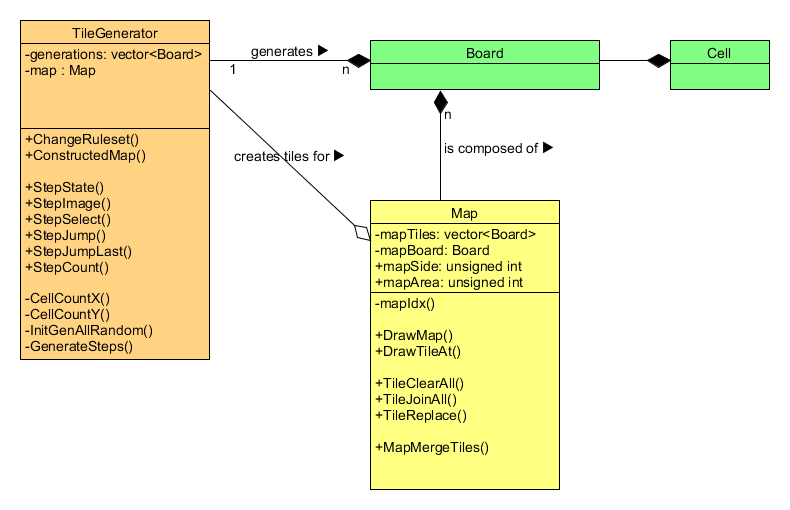
\includegraphics[width=0.9\linewidth]{diagrams/tilegenerator_map}
	\caption{ A model of interactions between TileGenerator, Board and Map classes. Source: own work}
	\label{fig:tilegeneratormap}
\end{figure}

The $Map$ class represents its state in two ways - as a collection of $Board$ states and as a single $Board$ instance with dimensions equal to tile width and height multiplied by their count along the Map borders - for example, a square map composed of 25 tiles with 64 by 128 size would have a width of 320 and a height of 640. Such dual representation allows the user to switch between two views onto the map - a tile grid view and a complete map view.

\subsubsection{Basic operations}

Initializing the first $Board$ contained in $TileGenerator$ class with random states enables the generator to use it as a base for further transformations, while also ensuring that each generated tile will be different. The operation used to do so is the $InitGenAllRandom$ method contained in $TileGenerator$.

After the initial state of the $Board$ is prepared, $TileGenerator$ can then use $GenerateSteps()$ method to create $Board$ states following the initial one by applying operations defined in and selected by current $Ruleset$. 
 
Copying a tile state from the $TileGenerator$ collection to the $Map$ grid requires user interaction. Any tile in the window showing the current $Map$ state can be clicked by the user, which invokes the $TileReplace()$ method of the $Map$ class, effectively copying the tile state visible in the tile generation window to the map grid.

Drawing cell states in tile generation and map grid windows is achieved by the $Board$ class method, $DrawCellsToTexture()$, described previously. Additionally, $Map$ provides operations for drawing its state depending on the selected view mode - $DrawMap()$ and $DrawTileAt()$.

\subsubsection{Merging tiles}

\td{result: generated random board after X transform steps becomes a useful tile}

The process of merging generated tiles into a map consists of two steps and requires user interaction. Once the map designer decides that tile prepared in the generation window is a sufficient candidate to be used in a map, its state can be copied to the map grid by clicking on one of the tiles in map window. Such action overwrites all cell states in the map tile with those contained in the prepared tile.

The second step of merging tiles is to ...



\subsection{User interface}

\td{ how designers can get a complete map model? }   

\begin{figure}[h]
	\centering
	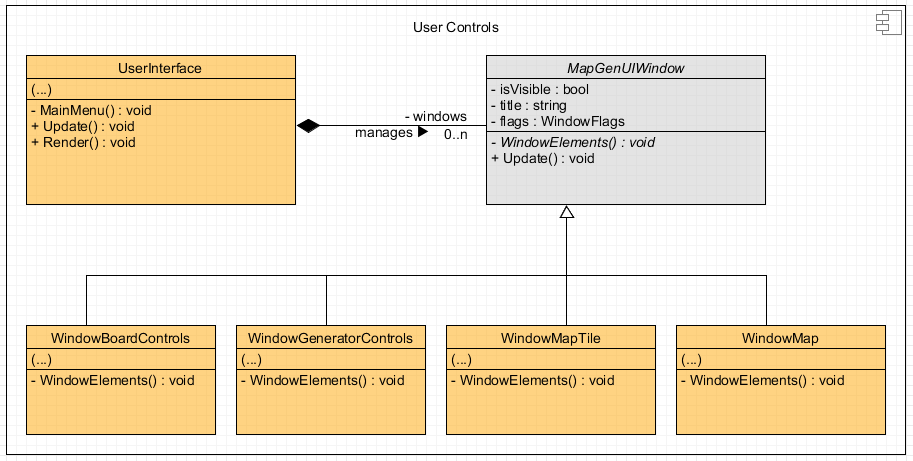
\includegraphics[width=0.8\linewidth]{diagrams/uiwindows}
	\caption[User Interface model]{A model of classes representing the user interface in the map generator program. Source: own work}
	\label{fig:uiwindows}
\end{figure}

\td{ exporting data from generator? }

%%%%%%%%%%%%%%%
\section{Experiments in generating maps with CA}

After implementing the map generator, it is possible to carry out experiments to find the optimal parameter ranges for map generation.

\begin{figure}[h]
	\centering
	\begin{subfigure}[b]{0.4\textwidth}
		\centering
		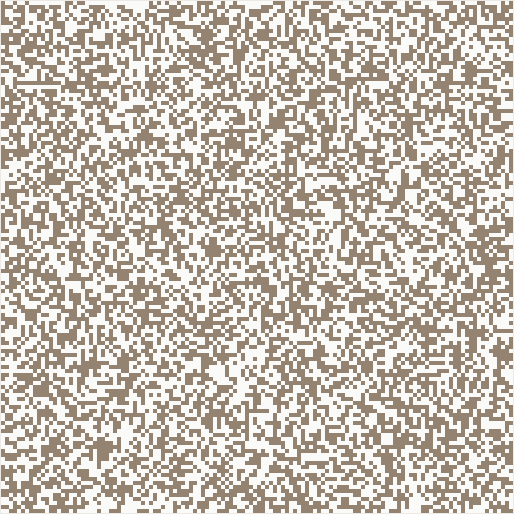
\includegraphics[width=\textwidth]{images/step1}
		\caption{Step 1 - random noise} 
	\end{subfigure}
	\hfill
	\begin{subfigure}[b]{0.4\textwidth}
		\centering
		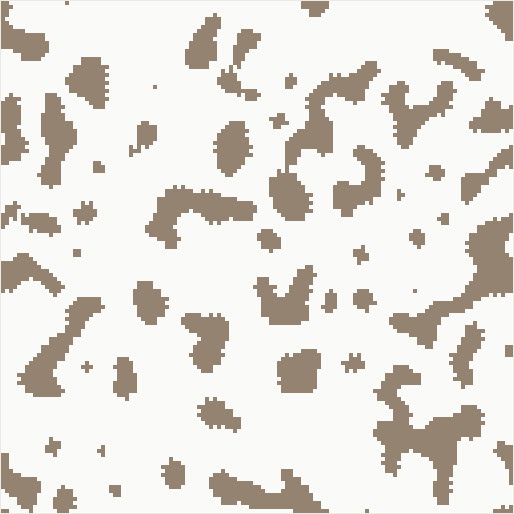
\includegraphics[width=\textwidth]{images/step2}
		\caption{Step 2 - generated tile} 
	\end{subfigure}
	\hfill
	\begin{subfigure}[b]{0.4\textwidth}
		\centering
		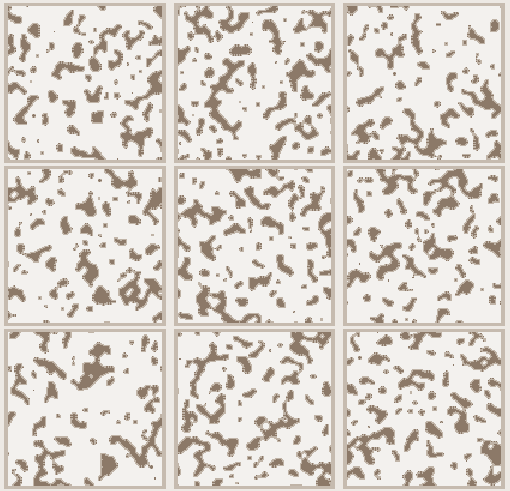
\includegraphics[width=\textwidth]{images/step3}
		\caption{Step 3 - tiles in a grid} 
	\end{subfigure}
	\hfill
	\begin{subfigure}[b]{0.4\textwidth}
		\centering
		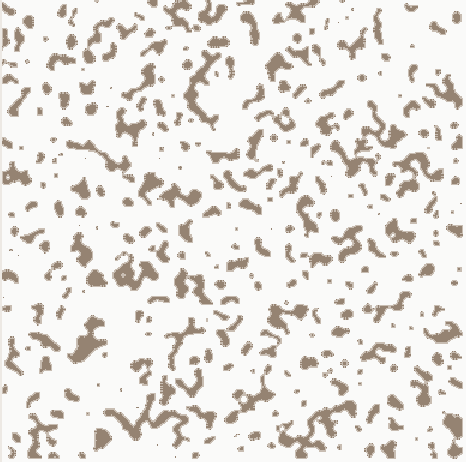
\includegraphics[width=\textwidth]{images/step4}
		\caption{Step 4 - complete map} 
	\end{subfigure}
	\caption{Four stages of map construction}
	\label{fig:map_steps}
\end{figure}



%%%%%%%%%%%%%%%%%%%%%%%%%%%%%%%%%%%%%%%%%%%%%%%%%%%%%%%%%%%%%%%%%%%%%%%%%%%%%%%%%%%%%%%%%%
\chapter{Conclusions} \label{rozdzial.podsumowanie}
%%%%%%%%%%%%%%%%%%%%%%%%%%%%%%%%%%%%%%%%%%%%%%%%%%%%%%%%%%%%%%%%%%%%%%%%%%%%%%%%%%%%%%%%%%

\td{Co do conclusion to prosze zebrać wnioski, nie przemyślenia, z całego 
	tego projektu i opisać wady i zalety Pana rozwiązania. Czemu jest inne 
	niz wszystkie co wprowadza nowego a co starego naprawia.}

\td{mention Bret Victor talks, why we choose ImGui, usefulness of Immediate Mode }

%%%%%%%%%%%%%%%
\section{Evaluation of results} 

\subsection{Effectiveness}  

%%%%%%%%%%%%%%%
\section{Possible improvements}

\td{future: expanding the generator}
At this point, we could also observe a common property of cellular automata  - whenever cell states need to change (the simulation moves to a later step), the state change is applied to every cell in the grid before simulation step ends \autocite{wolfram1984cellular} and cells do not need to be updated in sequence if only all cells will be changed before the next step. Hence, cell state updates could be applied in parallel to reduce the time needed to compute the simulation step. One way to do so would be to apply the findings presented by Reno Fourie in his thesis about applying CUDA technology to reduce time to compute next state of the board in case of 2-dimensional cellular automata \autocite{fourie2015parallel}. 

\td{future: adding more rules}
\td{future: user defined cell types}
\td{future: non-discrete cell states or more complex cell types }
\td{future: 3d maps?}

\td{Showing each step of image transformation could be useful to the designer, allowing them to control what kind of generated tiles will be chosen to compose the map. }

\td{Another potentially useful feature would be manual editing of tiles before they are placed in the map, which would allow for an even greater degree of control over tile contents. Further expansion of such feature could be to provide the designer with tools to make their own rules for tile generation, while also allowing them to define types of single cells composing the tile.}

\td{Although saving or exporting maps is not really necessary for experimentation and testing, a production version of the program should have such functionality. Finally, a map generator without a mechanism for saving the work done by a designer would certainly not be a useful tool. Such program needs a way to export generated maps to a file format that later can be used by a game engine of choice, possibly with procedures written by other programmers. }

%%%%%%%%%%%%%%%%%%%%%%%%%%%%%%
%%% KONIEC PRACY %%%%%%%%%%%%%
%%%%%%%%%%%%%%%%%%%%%%%%%%%%%%
\printbibliography[heading=bibintoc]

\addcontentsline{toc}{chapter}{List of figures} 
\listoffigures

\addcontentsline{toc}{chapter}{List of tables} 
\listoftables 

\addcontentsline{toc}{chapter}{Attachments} 
%%%%%%%%%%%%%%%%%%%%%%%%%%%%%%
\chapter*{Attachments}
\begin{enumerate} 
\item \td{include thesis defence documents}
\item \td{attach 1}
\item \td{attach 2}
\item \td{attach 3}
\end{enumerate} 

\end{document}
